\documentclass[12pt]{article}
\usepackage[utf8]{inputenc}
\usepackage[T1]{fontenc}
\usepackage{amsmath,amssymb,tikz-cd,tikz}
\usepackage{geometry}
\geometry{margin=2.5cm}

\begin{document}

\begin{center}
\textit{-- 3 --}
\end{center}

\noindent\underline{Ex}/ \quad 1) Calculaţi $(S_n)'$.

\bigskip
\noindent 2) Dacă $G\xrightarrow{\ \varphi\ } \dfrac{G}{G'} = G^{ab}$

\[
\begin{tikzcd}[column sep=large, row sep=large]
G \arrow[dr,"f"'] \arrow[r,"\varphi"] & G^{ab} \arrow[d, dashed, "\bar f"] \\
& \Gamma
\end{tikzcd}
\]

\noindent $\Gamma$ gr.\ abelian.

\noindent $(\exists!)\,\bar f$ morfism a.î.\ $f = \bar f\circ\varphi$

\bigskip
\noindent $\varphi$ morfism canonic

\noindent $f$ morf.\ de gr.

\bigskip
\begin{center}
\underline{\textbf{Grupul diedral $D_n$, $n\geq 3$}}
\end{center}

\bigskip
\noindent $x' = R\cos(t+\alpha)$

\noindent $y' = R\sin(t+\alpha)$

\begin{center}
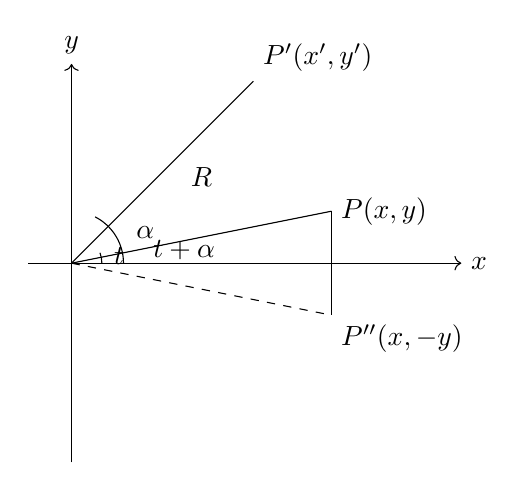
\begin{tikzpicture}[scale=1.1]
\draw[->] (-0.5,0) -- (4.5,0) node[right] {$x$};
\draw[->] (0,-2.3) -- (0,2.3) node[above] {$y$};
\coordinate (O) at (0,0);
\coordinate (P) at (3,0.6);
\coordinate (Pp) at (2.1,2.1);
\coordinate (Pdp) at (3,-0.6);
\draw (O) -- (P) node[right] {$P(x,y)$};
\draw (O) -- (Pp) node[above right] {$P'(x',y')$};
\draw (P) -- (Pdp);
\draw[dashed] (O) -- (Pdp) node[below right] {$P''(x,-y)$};
\draw (0.6,0) arc (0:63:0.6);
\node at (0.85,0.35) {$\alpha$};
\draw (0.35,0) arc (0:20:0.35);
\node at (0.55,0.08) {$t$};
\node at (1.3,0.15) {$t+\alpha$};
\node at (1.5,1.0) {$R$};
\end{tikzpicture}
\end{center}

\noindent $R = \sqrt{x^2+y^2} = \sqrt{x'^2+y'^2}$

\bigskip
\noindent
\[
\begin{pmatrix}x'\\y'\end{pmatrix} = \begin{pmatrix}\cos\alpha & -\sin\alpha\\ \sin\alpha & \cos\alpha\end{pmatrix}\begin{pmatrix}x\\y\end{pmatrix}
\]

\noindent $\underbrace{R_\alpha}_{} \in M_2(\mathbb{R})$

\bigskip
\noindent
\[
\begin{pmatrix}x\\-y\end{pmatrix} = \begin{pmatrix}1&0\\0&-1\end{pmatrix}\begin{pmatrix}x\\y\end{pmatrix}
\]

\noindent $\underbrace{S}_{}\in M_2(\mathbb{R})$

\bigskip
\noindent\underline{Def} \ Fie $G\leq GL_2(\mathbb{R}) = \{A \mid A\in M_2(\mathbb{R}) \text{ cu } \det A\neq 0\} =$

\noindent = gr.\ general liniar de grad 2 peste $\mathbb{R}$

\bigskip
\noindent
\[
R_{\frac{2\pi}{n}} = \begin{pmatrix}\cos\frac{2\pi}{n} & -\sin\frac{2\pi}{n}\\[4pt] \sin\frac{2\pi}{n} & \cos\frac{2\pi}{n}\end{pmatrix}
\qquad
S=\begin{pmatrix}1&0\\0&-1\end{pmatrix}
\]

\bigskip
\noindent $\Big\langle R_{\frac{2\pi}{n}},\,S\Big\rangle = D_n$ şi s.n.\ \underline{grupul diedral $D_n$}, $n\geq 3$

\bigskip
\noindent\underline{Prop.} \ $D_n$ e un gr.\ cu $2n$ elem.; \ ord $R=n$ \ $\big(R=R_{\frac{2\pi}{n}}\big)$

\noindent ord $S=2$ şi $SR=R^{n-1}S$

\bigskip
\noindent\underline{Teoremă}: \ Fie $G$ un gr.\ a.î.\ $\exists\,a,b\in G$ cu prop.

\begin{enumerate}
\item[1)] $\langle a,b\rangle = G$
\item[2)] ord $a=n$, $n\geq 3$, ord $b=2$ şi $ba=a^{n-1}b$
\end{enumerate}

\noindent Atunci $G\cong D_n$ şi ord $G=2n$

\end{document}
